\documentclass[twoside,11pt]{article}

% Any additional packages needed should be included after jmlr2e.
% Note that jmlr2e.sty includes epsfig, amssymb, natbib and graphicx,
% and defines many common macros, such as 'proof' and 'example'.
%
% It also sets the bibliographystyle to plainnat; for more information on
% natbib citation styles, see the natbib documentation, a copy of which
% is archived at http://www.jmlr.org/format/natbib.pdf

\usepackage{jmlr2e}
\usepackage{graphicx}
\usepackage{tabularx}
\usepackage{booktabs}
\usepackage{wrapfig}
\usepackage{amsmath}
\usepackage{chngcntr}
\usepackage{relsize}

\counterwithin{figure}{section}
\counterwithin{table}{section}
\setlength{\extrarowheight}{3pt}
% Definitions of handy macros can go here

\newcommand{\dataset}{{\cal D}}
\newcommand{\fracpartial}[2]{\frac{\partial #1}{\partial  #2}}

% Short headings should be running head and authors last names

\ShortHeadings{Comparison of Feed-Forward and Gaussian Neural Networks}{Brekke, Wall, et. al.}
\firstpageno{1}

\begin{document}
	
	\title{Review of the Capabilities of Multi-Layer Perceptrons and Gaussian Radial Basis Function Neural Networks on Categorization and Regression Data}
	
	\author{\name Kyle J Brekke \email brekke.kylej@gmail.com \\
		\addr Gianforte School of Computing\\
		Montana State University\\
		Bozeman, MT 59717-2220, USA
		\AND
		\name Ren H. Wall \email renwall@protonmail.ch \\
		\addr Gianforte School of Computing\\
		Montana State University\\
		Bozeman, MT 59717-2220, USA
		\AND
		\name Nicholas J. Rust \email  nicholasrust@protonmail.com \\
		\addr Gianforte School of Computing\\
		Montana State University\\
		Bozeman, MT 59717-2220, USA
		\AND
		\name Alexander Mershon \email alexdavidmershon@gmail.com \\
		\addr Gianforte School of Computing\\
		Montana State University\\
		Bozeman, MT 59717-2220, USA}
	
	\editor{Kyle J Brekke}
	
	\maketitle
	
	\begin{abstract}
		In this paper we compare the performance of feed forward and radial basis function (RBF) neural networks on regression and classification. We use multiple feed forward networks with different hidden layers and multiple RBFs trained on multiple different clustering and reduction methods.
		We use a collection of six datasets from the UCI Machine Learning Archive to test our results.
		Three of these datasets have categorical classes, whereas the other three are regression datasets. For classification datasets we collect accuracy and for regression datasets we collect the mean actual error. After collecting all our measurements we find that there is a significant improvement from the best Feed Forward network to the best RBF network, except in the machine data set where we are unable to draw conclusions. 
	\end{abstract}
	
	\begin{keywords}
		Machine Learning, Radial Basis Function, Backpropogation, Classification, Regression, Feed-Forward, k-Nearest Neighbors, Condensed Nearest Neighbors, k-Means Clustering, Partitioning Around Medoids
	\end{keywords}
	
	% The content of each section should be in the file for that section.
	% When defining new sections please do so in a new file and \input it here.
	

\section{Introduction}\label{sec:introduction} The purpose of this project is to analyze feed-forward and radial basis function neural networks for classification and regression tasks. This will be done by comparing the performance of the feed-forward network with 0, 1, and 2 hidden layers and the RBF using the results of condensed nearest neighbor, k-means clustering, and k-medoids clustering as the locations for its basis functions. The performance of each will be analyzed across each of the six datasets. For classification datasets we collect the accuracy and error, while we collect mean actual error for regression sets.


	
	\subsection{Hypotheses}
For feed-forward networks, we hypothesize that their performance will decrease as the number of their hidden layers increases. For radial basis function networks, we believe that condensed will provide the best performance, k-medoids will provide the second best performance, and k-means will result in the worst performance of the three. Further we hypothesize that for each dataset we will see a significant difference between the best of each type of model (i.e. the highest performing feed forward variation will be significantly better then the highest performing RBF model, or vice versa).
	
	\section{Implementation}\label{sec:implementation}

\subsection{Feed-Forward Neural Network}

Feed-forward networks, otherwise referred to as multi-layer perceptrons, have three primary components: an input layer, zero-to-many hidden layers, and an output layer \citep{Fine1999}. Each layer contains a set of neurons which interact with an input vertex via a weighting vertex and activation function (Figure 2.1). For our implementation, the input layer has been abstracted such that it does not actually contain any neurons. Neurons in the hidden layers apply weights to the input vector, which is then passed to a logistic activation function (Equations 1 and 2).

\begin{equation}
a_h = w^T_h\hat{x}
\end{equation}

Where $w^T_h$ is the weight vector for neuron $h$, and $\hat{x}$ is the input vector $\{x_1, x_2, ..., x_M\}$. From the created value $a_h$, hidden layer neurons can then calculate their output values $z_h$.

\begin{figure}[b!]
	\centering
	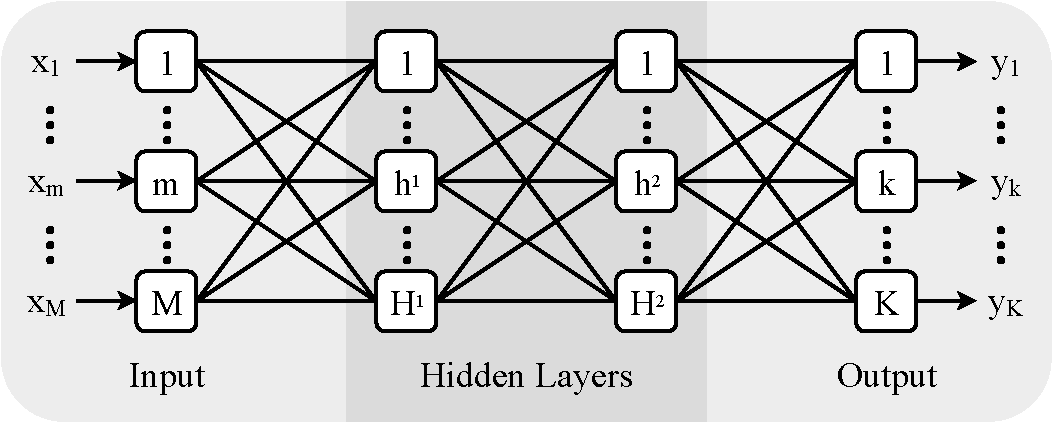
\includegraphics[width=0.9\linewidth]{images/feed_forward_diagram.pdf}
	\caption{Generic diagram of a feed-forward network with two hidden layers, where there are $M$, $H_1$, $H_2$, and $K$ neurons in each layer.}
\end{figure}

\begin{equation}
z_h = \frac{1}{1 + \text{exp}\left({-a_h}\right)}
\end{equation}

\bigbreak
If the network is used for a classification set, the output layer will also use this method for generating its outputs (where there will be an output neuron for each $k$ possible classifications, where the largest output determines the classification of the input) whereas regression sets will use a single linear activation function, which simply returns $y_k = a_k = w^T_k\hat{x}$ as an estimation of the actual value of the input.

When training a feed-forward network, our model takes in a training set, and then performs forward propagation, followed by back propagation. In forward propagation, the first layer takes in the features of the training row, then each proceeding layer takes in a vector of the previous layer's results until reaching the output layer. The resulting vector of the output layer is the result of forward propagation. We then perform back propagation using this result, where we calculate a change in weighting values using stochastic gradient descent. For this, we have two cost functions which correspond to the output layer (Equation 3) and all preceding layers (Equation 4):

\begin{equation}
	\delta_k = r_k - y_k
\end{equation}
\begin{equation}
	\delta_h = z_h(1 - z_h)\mathlarger{\mathlarger{\Sigma}}_{_i}(\delta_i)
\end{equation}

\bigbreak
Where $\delta_i$ is the cost for the $i$th neuron in the following layer and $r_k$ is the expected output for a given output neuron $k$. For categorization, $r_k$ is 1 if the input values are from the class of the corresponding output neuron and 0 otherwise, while $r_k$ is the actual value of the input entry in regression sets. For each neuron $n$ in the network, their weights are then updated using the following equations:

\begin{equation}
\Delta_i = (\eta\delta_i)\hat{x}
\end{equation}
\begin{equation}
	w_i = w_i + \Delta^\phi_i + \alpha\Delta^{\phi - 1}_i
\end{equation}

\bigbreak
Where $\eta$ and $\alpha$ are tuned constants which correspond to the learning rate and momentum of the network, and $\phi$ is the current iteration of back propagation. The learning rate is used to dampen the impact of the changes made, so that any given category being trained is not over-emphasized during classification, while momentum is used to add a portion of the previous epoch of back propagation onto the current changes, such to continue a 'trend' towards an optimized weight.

Back propagation is then repeated until convergence (when the output of the network ceases to change on further iterations) or until an arbitrary loop threshold has been met. Once this process of forward and back propagation has been repeated for every entry in the training dataset, the network is considered 'trained' and can be used to classify new inputs.

\subsection{Radial Basis Function Neural Network}

Radial basis function (RBF) networks operate similarly to feed forward networks, with an input layer, intermediary layer, and output layer. The notable difference between the two networks is that in and RBF network there is always one layer between the input and output layers (Figure 2.2)\citep{Fernandez2012}. Neurons in the intermediary layer also use a radial basis function rather than a sigmoid function for activation. For our purposes, neurons in our implementation use a Gaussian basis function (Equation 7).

\begin{figure}[t!]
	\centering
	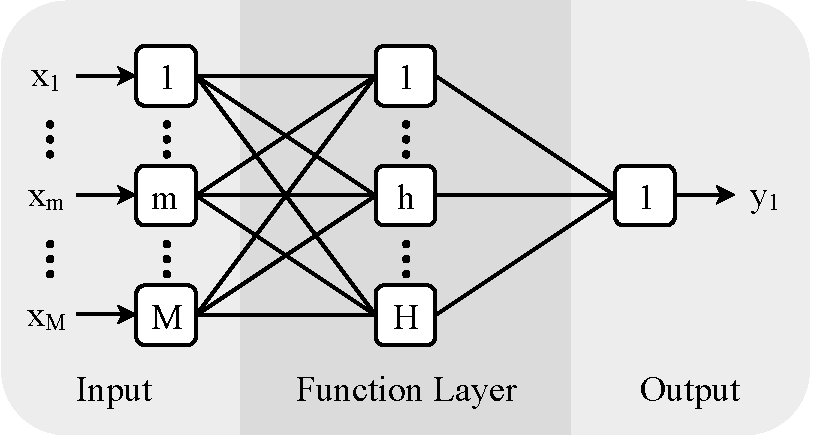
\includegraphics[width=0.7\linewidth]{images/radial_basis_function_diagram.pdf}
	\caption{Generic radial basis function (RBF) neural network with $M$ inputs, $H$ Gaussian basis function neurons, and one output neuron.}
\end{figure}

\begin{equation}
z_h = \text{exp}{\left(-\frac{(\|\hat{x} - c_h\|)^2}{r^2_h}\right)}
\end{equation}

Where $c_h$ is the 'center' -- or prototype -- of the neuron $h$, and $r_h$ is the kernel width of the neuron's function. The $c_h$ of each neuron is determined using the values of the training set passed to the network, while the $r_h$ is calculated using the distance between the function's center and its closest neighbor (Equation 8)\citep{Nabil2003}.

\begin{equation}
	r = ||c_n - c_h||
\end{equation}

Where $c_n$ is the center of the center of the nearest neighbor to $c_h$.

There are several methods for selecting the centers and number of neurons, each of which relies on reducing the initial training dataset into a smaller essential training set. For our purposes, we applied three of these methods: condensed nearest neighbor, k-means clustering, and partitioning around medoids.

\subsubsection{The k-Nearest Neighbors Algorithm}

The k-nearest neighbors algorithm is the foundation of all methods of RBF training set reduction we employ in this project. Given a labeled training set, the algorithm is able to classify other data entries into one of the given labels. K-nearest neighbor is a 'lazy learner', which means it does not require any training calculations to be performed on the training set for it to be able to classify other data. For our purposes, distances between vectors is calculated using L2 norm, from which the associated Frobenius norm yields the Euclidean distance \citep{GolubGeneH.GeneHoward1989Mc}, represented as:

\begin{equation}
	D\langle v, v' \rangle = \sqrt{\sum_{i=1}^{n}|v_i - v_i'|^2}
\end{equation}

Where $D\langle v, v' \rangle$ is the Euclidean distance between two vectors $v$ and $v'$, and $v_i, v_i'$ are the $i^{\text{th}}$ values of $v$ and $v'$ respectively.

\subsubsection{Condensed Nearest Neighbor}

The condensed nearest neighbor algorithm begins with an empty 'condensed' set which it adds values to from the training set. Condensed nearest neighbor determines which data entries will be added to the set by classifying each entry in the training set using its nearest neighbor in the existing condensed training set. If an entry is not correctly classified, then it is considered essential and added to the condensed set. An entry is considered non-essential and discarded if it is categorized correctly. After performing this operation for all entries in the original training set, the condensed nearest neighbor algorithm returns the finalized condensed training set for use by the radial basis function network.

\subsubsection{Clustering by Means}

The k-means clustering algorithm seeks to find approximate centroids of subsets within the training data by creating \textit{k} random points in the data's feature space, and then continuously adjusting them in order to minimize the total overlap of data points between clusters \citep{Mirkin1996}. The algorithm terminates when all points 'settle' and further iterations no longer result in changes to the centroids. Once centroids which do not encompass any of the training data are removed, the remaining centroids are used as a reduced training set for our network.

\subsubsection{Partitioning Around Medoids}

Partitioning around medoids operates on a similar principal to k-means clustering, with a few key differences \citep{Farcomeni2016}. Instead of being randomly generated within the feature space, medoids are selected from entries in the training set. This is true when the points are adjusted as well; when the medoids are shifted, they are moved to a new point in the training set. Additionally, medoids do not determine their clusters through mean, but instead through their nearest neighbors. Medoids are batch updated by calculating the distortion of swapping each medoid with each point in its respective cluster then selecting the swap with the lowest distortion for each medoid. As a result of how medoids are selected, we do not need to purge any of medoids from the reduced training set once the algorithm terminates.

	
	\section{Experimental Approach}\label{sec:experimental-approach}

\subsection{Data Preprocessing}

We will be testing six datasets -- \textit{car}, \textit{wine quality} \citep{CCAMaR2009}, \textit{abalone}, \textit{forest fires} \citep{CaM2007}, \textit{machine}, and \textit{segmentation} -- from the UCI Machine Learning Archive (Table 3.1), which can be divided into one of two categories: classification and regression. Classification datasets are categorical in nature, with each entry in a classification set belonging to one of several possible categories. Regression sets are continuous, where each entry corresponds to a specific real-value, instead of a broad category \citep{Dua:2019}. 

Before experimentation begins, we first perform preprocessing on each dataset. Of note, irrelevant or unusable data are dropped, such as features which are the same for every entry or have random, non-quantifiable values. Additionally, non numeric values in datasets which can be quantified are converted, either by applying gradient integer values to the features, or breaking a feature into many binary fields for each possible value in the original feature. Finally, all data are normalized at the end of preprocessing, such that every feature value falls between 0 and 1.

\begin{table}[b!]
	\centering
	\begin{tabularx}{1\linewidth}{| c | X | X | X | X | X | X |}
		\hline
		Type 			& \multicolumn{3}{c|}{Categorical}	& \multicolumn{3}{c|}{Regression} 			\\ 
		\hline
		Dataset 		&$Abalone$    &$Car$ 		 &$Segment.$&$Machine$ &$Wine$ $Quality$& $Forest$ $Fires$\\ 
		\hline
		Training 		&3772		  &1557			 &189		  &189		   &5848		 &466		 \\ 
		\hline
		Validation		&405		  &171			 &21		  &20		   &649			 &51		  \\ 
		\hline
		\textbf{Total}	&\textbf{4177}& \textbf{1728}&\textbf{210}&\textbf{209}&\textbf{6497}&\textbf{517}\\ 
		\hline
	\end{tabularx}
	\caption{Experimental data organized by type, broken down by subset size.}
\end{table}

\subsection{Testing Procedures}
Once a dataset has been processed, it is separated into a training and validation subset, where the training subset is roughly 90\% of the original dataset, and the validation set is the remaining 10\% (Table 3.1). Once this has been accomplished for all datasets, each dataset will then be trained and validated on several variations of feed-forward and radial basis function network. 

Classification datasets will be tested on feed-forward networks with 0, 1, and 2 hidden layers where each hidden layer has as many neurons as features in the dataset, as well as RBF networks which have their neurons determined using reduced training sets created through the use of condensed nearest neighbor, k-means clustering, and partitioning around medoids, where the number of initial clusters in k-means and medoids is determined by the size of the reduced dataset created by condensed nearest neighbor. Regression datasets will be tested on the same variations, with the exception of the condensed nearest neighbor variant of the radial basis function network. The number of initial clusters for k-means and medoids have therefore been determined to be one quarter of the size of the original training set. 

Learning rate and momentum have been tuned prior to testing. A range of learning rates $0.01 \leq \eta \leq 0.5$ and momentum values $0.01 \leq \alpha \leq 0.5$ were tested during the development of our model, finding that a learning rate of $\eta = 0.1$ and momentum of $\alpha = 0.05$ yielded our best results.

Once all datasets have been tested, their results will be analyzed according to their type. Classification datasets will be measured using micro-averaged accuracy. Regression sets will be measured using mean average error (MAE)\citep{Chai2014}. The significance of our results will then be evaluated using a test of proportions \citep{Dietterich1997}.

\begin{equation}
	z = \frac{\rho_A - \rho_B}{\sqrt{2\rho(1 - \rho) / N}}
\end{equation}

\bigbreak
Where $\rho_A$ is a loss function for model A, $\rho_B$ is the same loss function for model B, and $\rho = \frac{\rho_A + \rho_B}{2}$. The calculated $z$ value can then be used to determine the significance of results via a statistical Z-test.

	
	\section{Results and Conclusions}

After testing every dataset on each of our models, we are able to observe a number of trends. In classification datasets, there is a distinct difference in classification accuracy between feed-forward and RBF networks. All three of our classification datasets showed greater performance when classified using an RBF network. Additionally, the prediction accuracy of feed-forward models consistently decreased as the number of hidden layers increased (Figure 4.1).

In regression datasets, the addition of hidden layers seems to result in reduced error in feed-forward networks, as networks with one hidden layer displayed lower mean actual error for every regression dataset tested when compared to the results of the same validation and training set on a feed-forward network with no hidden layers, though error appears to increase again when networks have two hidden layers (Figure 4.2).

Although the performance changes which result from additional hidden layers appear to vary based on whether the dataset tested was a classification or regression set, the highest performance was seen unanimously in one of the RBF models in every experiment.

\begin{figure}[b]
	\centering
	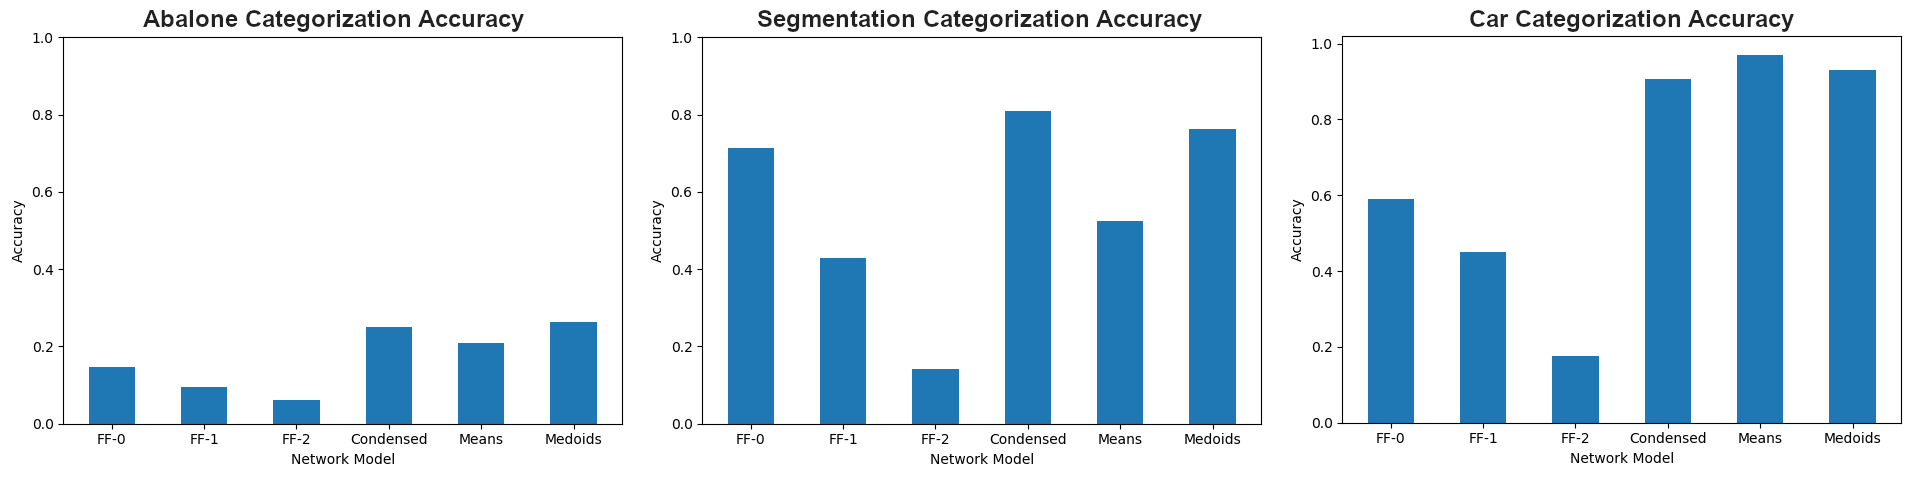
\includegraphics[width=\linewidth]{images/classification_results.png}
	\caption{Accuracy for each model applied to each regression dataset.}
\end{figure}

\begin{figure}[t]
	\centering
	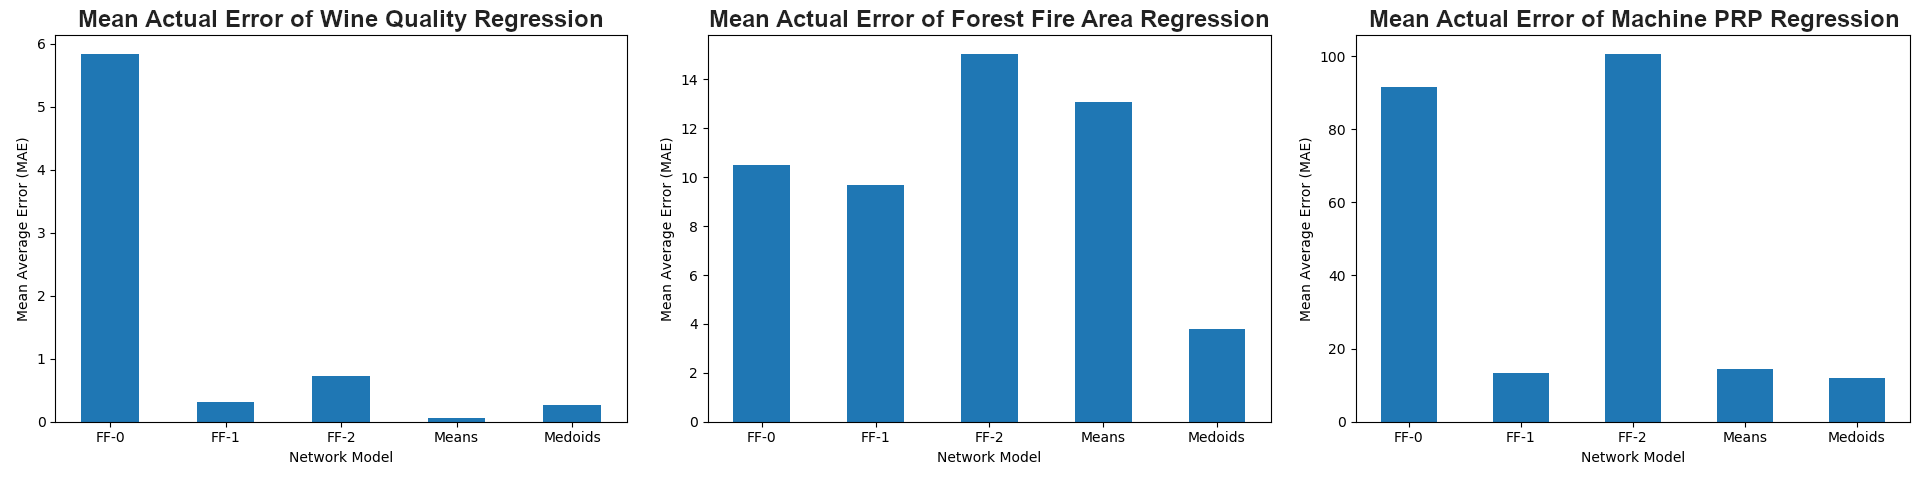
\includegraphics[width=\linewidth]{images/regression_results.png}
	\caption{Mean actual error for each model applied to each regression dataset.}
\end{figure}

\pagebreak

\begin{table}[t]
	\begin{tabularx}{\linewidth}{|c|X|X|X|X|X|X|}
		\hline
		Dataset & \textit{Abalone} & \textit{Car} & \textit{Segment.} & \textit{Machine} & \textit{Wine Quality} & \textit{Forest Fires} \\
		\hline
		$z$ Statistic & 27.392 & 8.587 & 6.228 & 0.0311 & 25.177 & 19.601 \\
		\hline
		$p$ Value & $<$ 0.00001 & $<$ 0.00001 & $<$ 0.00001 & 0.48759 & $<$ 0.00001 & $<$ 0.00001 \\
		\hline
	\end{tabularx}
	\caption{$z$ statistics and corresponding $p$ values for the difference in performance observed from the highest performing feed-forward and radial basis function variations in each dataset.}
\end{table}

In order to generally compare the feed-forward and radial basis function models for each dataset, we performed significance calculations on the highest performing variant for both models (Table 4.1). For all datasets but the \textit{machine} set, we are able to observe that the difference in performance was statistically significant within a confidence interval of 99.99\%. The difference in performance observed in the machine dataset can not be considered statistically significant within any reasonable confidence interval ($<$ .10).

From the results of our significance calculations, we are able to conclude that the performance of our radial basis function network was superior to the performance of our feed-forward network for the \textit{abalone}, \textit{car}, \textit{segmentation}, \textit{wine quality}, and \textit{forest fires} datasets. 



	
	\section{Summary}\label{sec:summary}
In this paper we compared the performance of feed forward and RBF neural networks on regression and classification.
For each of our six datasets we trained three feed forward networks with 0, 1, and 2 hidden layers and three RBF networks with datasets reduced using condensed nearest neighbor, k-means clustering, and partitioning around medoids.
After calculating accuracy and error for each network we were able to come to conclusions concerning the relative performance of the two network types. 
Through our results, we were able to determine that the highest performing variation of RBF network was significantly better than the highest performing variation of feed forward network in all datasets except \textit{machine}.
	
	\newpage
	\vskip 0.2in
	\bibliography{bibliography}
	
\end{document}
